\chapter{Optimization Techniques/ Optimizers}

\section*{Notation}

\begin{table}[h]
    \begin{tabular}{l l}
        $\mathbf{x}$ / $\mathbf{w}$ & input/ parameters \\
        
        $L$ / $Q$ / $E$ & Loss Function/ Cost Function \\

        $\nabla L(\mathbf{x})$ / $\nabla Q(\mathbf{w})$ & Gradient of $L(\mathbf{x})$ wrt $\mathbf{x}$ \\
    \end{tabular}
\end{table}


\section{Gradient Descent/ Stochastic Gradient Descent (SGD) \cite{wiki-Gradient_descent,wiki-Stochastic_gradient_descent}}\label{Gradient Descent (GD)}\label{Stochastic Gradient Descent (SGD)}

\begin{table}[h]
    \begin{minipage}[t]{0.5\linewidth}
        \begin{figure}[H]
            \centering
            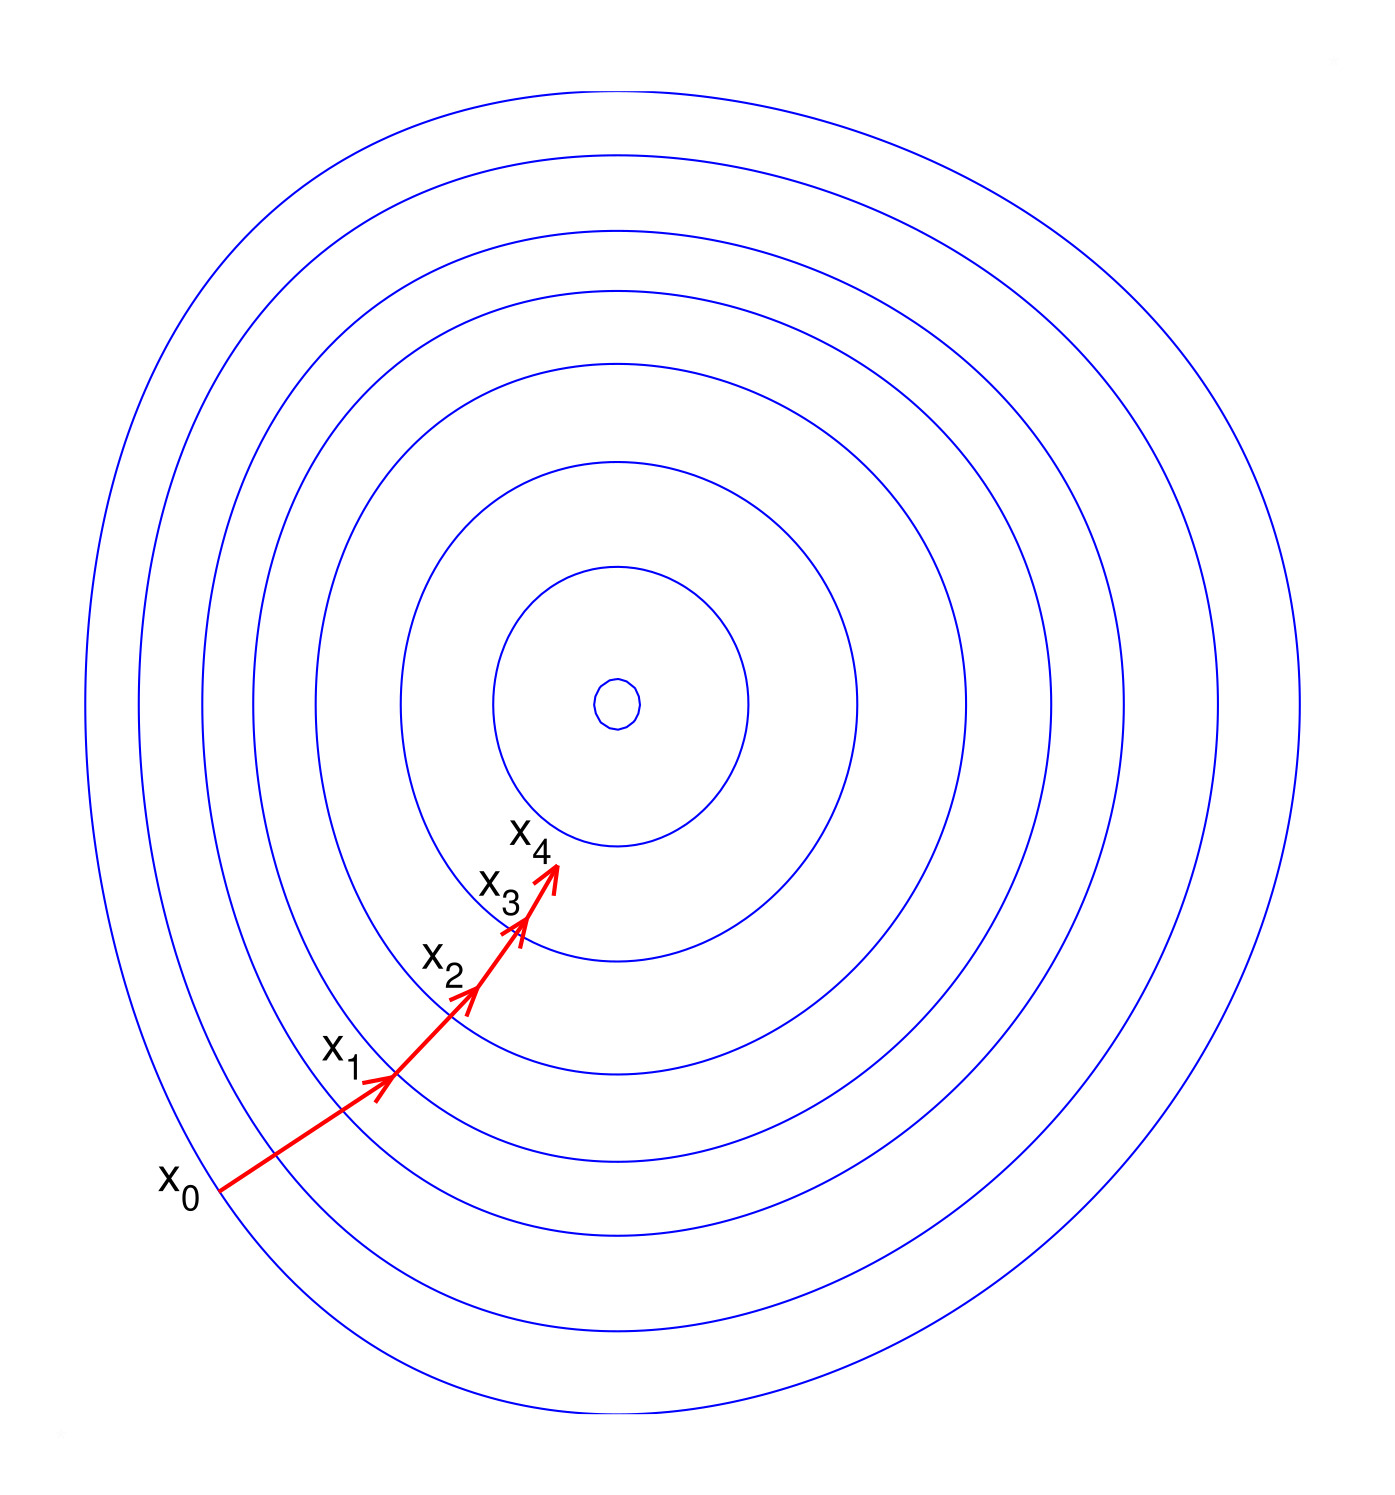
\includegraphics[width=\linewidth, height=3.5cm, keepaspectratio]{Pictures/optimizers/Gradient_descent.jpg}
            \caption{Gradient Descent (SGD)}
        \end{figure}
    \end{minipage}
    \hfill
    \begin{minipage}[t]{0.5\linewidth}
        \begin{itemize}
            \item Gradient descent is a method for \textbf{unconstrained} mathematical optimization. 
            
            \item It is a \textbf{first-order iterative algorithm} for finding a local minimum of a differentiable multivariate function.
        \end{itemize}        
    \end{minipage}
\end{table}

\[
    \displaystyle \mathbf {x} _{n+1}=\mathbf {x} _{n}-\gamma _{n}\nabla F(\mathbf {x} _{n}) \hfill n\geq 0
\]


Stochastic gradient descent (often abbreviated SGD) is an \textbf{iterative} method for optimizing an objective function with suitable smoothness properties (e.g. differentiable or subdifferentiable).

\[
    \displaystyle x = x - \eta\nabla L_{i}(x)
\]

\begin{algorithm}
    \caption{Stochastic gradient descent (SGD)}
    
    Choose an \textbf{initial vector} of parameters ${\displaystyle w}$ and learning rate ${\displaystyle \eta }$

    \Repeat{approximate minimum is obtained}{
        Randomly shuffle samples in the training set\\
        \For{$i=1,2,\cdots,n$}{
            $\displaystyle x = x - \eta\nabla L_{i}(x)$
        }
    }
\end{algorithm}


\section{Implicit updates SGD (ISGD)}\label{Implicit updates SGD (ISGD)}
Stochastic gradient is evaluated at the next iterate rather than the current one
\[
    {\displaystyle w^{\text{new}}:=w^{\text{old}}-\eta \,\nabla Q_{i}(w^{\rm {new}})} 
    \hfill 
    {\displaystyle w^{\text{new}}:=\arg \min _{w}\left\{Q_{i}(w)+{\frac {1}{2\eta }}\left\|w-w^{\text{old}}\right\|^{2}\right\}}
\]


\section{Batch Gradient Descent 
    VS 
    Mini-Batch Gradient Descent
    VS 
    Gradient Descent (SGD) 
    \cite{chatgpt}
}

\begin{longtable}{|p{2.5cm}|p{4cm}|p{3.5cm}|p{3.5cm}|}
    \caption{
    Batch Gradient Descent 
    VS 
    Mini-Batch Gradient Descent
    VS 
    Gradient Descent (SGD) 
    }\\
    
    \hline
    \textbf{Aspect} & \textbf{Batch Gradient Descent} & \textbf{Mini-Batch Gradient Descent} & \textbf{Gradient Descent (SGD)} \\
    \hline
    \endfirsthead
    
    \hline
    \textbf{Aspect} & \textbf{Batch Gradient Descent} & \textbf{Mini-Batch Gradient Descent} & \textbf{Gradient Descent (SGD)} \\
    \hline
    \endhead
    
    \hline\endfoot
    \hline\endlastfoot
    
    \textbf{Definition} & Updates parameters after computing the gradient on the entire dataset & Updates parameters after computing the gradient on a small batch of data & Updates parameters for each training example \\
    \hline

    \textbf{Update Frequency} & Low (after the entire dataset) & Medium (after each mini-batch) & High (after each example) \\
    \hline
    
    \textbf{Computation Cost/ Update} & High & Medium & Low \\
    \hline
    
    \textbf{Memory Usage} & High & Medium & Low \\
    \hline
    
    \textbf{Convergence Speed} & Slow & Fast & Fast \\
    \hline
    
    \textbf{Stability of Updates} & Stable (low variance) & Moderate (reduced variance) & Noisy (high variance) \\
    \hline
    
    \textbf{Convergence} & Guaranteed to decrease cost function & More stable convergence than SGD & May not converge to the global minimum \\
    \hline
    
    \textbf{Practical Use} & Suitable for smaller datasets & Suitable for large datasets & Suitable for very large datasets \\
    \hline
    
    \textbf{Hardware Optimization} & Limited & Allows for parallel processing & Limited \\
    \hline
    
    \textbf{Escape Local Minima} & Less likely & Yes (benefits of both SGD and Batch) & Yes (due to noisy updates) \\
    \hline
    
    \textbf{Example Size} & Entire dataset & Mini-batch (subset of dataset) & Single example \\
    \hline
    
    \textbf{Efficiency} & Low for large datasets & High, balancing efficiency and performance & High for very large datasets \\
    \hline

\end{longtable}


\section{SGD with Momentum \cite{wiki-Stochastic_gradient_descent}}\label{SGD with Momentum}
Stochastic gradient descent with momentum remembers the update $\Delta w$ at each iteration, and determines the next update as a linear combination of the gradient and the previous update:
\[
    {\displaystyle \Delta w:=\alpha \Delta w-\eta \,\nabla Q_{i}(w)}
    \hfill
    {\displaystyle w:=w+\Delta w}
\]

\section{Adaptive gradient (AdaGrad) (2011) \cite{wiki-Stochastic_gradient_descent}}\label{Adaptive gradient (AdaGrad)}
AdaGrad (for adaptive gradient algorithm) is a modified stochastic gradient descent algorithm with per-parameter learning rate.

\[
    {\displaystyle G=\sum _{\tau =1}^{t}g_{\tau }g_{\tau }^{\mathsf {T}}}
    \hfill
    ({\displaystyle g_{\tau }=\nabla Q_{i}(w)})
    \hfill
    {\displaystyle G_{j,j}=\sum _{\tau =1}^{t}g_{\tau ,j}^{2}}
\]
\[
    {\displaystyle w:=w-\eta \,\mathrm {diag} (G)^{-{\frac {1}{2}}}\odot g} 
    \hfill \text{ or } \hfill
    {\displaystyle w_{j}:=w_{j}-{\frac {\eta }{\sqrt {G_{j,j}}}}g_{j}}
\]

\begin{itemize}
    \item learning rate = $\eta$

    \item Each $\{G_{(i,i)}\}$ gives rise to a scaling factor for the learning rate that applies to a single parameter $w_i$.

    \item Since the denominator in this factor, ${\displaystyle {\sqrt {G_{i}}}={\sqrt {\sum _{\tau =1}^{t}g_{\tau }^{2}}}}$ is the $l_2$ norm of previous derivatives, extreme parameter updates get dampened, while parameters that get few or small updates receive higher learning rates.    
\end{itemize}


\section{Resilient backpropagation (Rprop) (1992) \cite{wiki-Rprop,pytorch-Rprop,florian.github.io/rprop}}\label{Resilient backpropagation (Rprop)}

\[
    \displaystyle w_i^{(t)} = w_i^{(t - 1)} - \eta_i^{(t - 1)} * \operatorname{sgn}\left(\frac{\partial E^{(t -
    1)}}{\partial w_i^{(t - 1)}}\right)
    \hfill
    \text{\cite{florian.github.io/rprop}}
\]
\[
    \displaystyle \eta_i^{(t)} = \begin{cases}
    \min(\eta_i^{(t - 1)} * \alpha, \eta_{\max}) & \text{if } \displaystyle\frac{\partial E^{(t)}}{\partial w_i^{(t)}} * \displaystyle\frac{\partial E^{(t - 1)}}{\partial w_i^{(t - 1)}} > 0 \\
    \max(\eta_i^{(t - 1)} * \beta, \eta_{\min}) & \text{if } \displaystyle\frac{\partial E^{(t)}}{\partial w_i^{(t)}} * \displaystyle\frac{\partial E^{(t - 1)}}{\partial w_i^{(t - 1)}} < 0 \\
    \eta_i^{(t - 1)} & \text{otherwise}
    \end{cases}
    \hfill
    (\alpha > 1 > \beta) \text{ \cite{florian.github.io/rprop}}
\]


\begin{itemize}
    \item This is a \textbf{first-order} optimization algorithm.
\end{itemize}

\begin{algorithm}[h]
    \caption{Resilient backpropagation (Rprop) (1992) \cite{pytorch-Rprop}}

    \Comment{
        $\theta_0 \in \mathbb{R}^d$ (params)\\
        $f(\theta)$ (objective)\\
        $\eta_{+/-}$ (etaplus, etaminus)\\
        $\Gamma_{max/min}$ (step sizes)
    }
    
    \SetKwFunction{FRprop}{Rprop}
    \SetKwProg{Fn}{Function}{:}{}
    \Fn{\FRprop{$\theta_0, f(\theta), \eta_{+/-}, \Gamma_{max/min}$}}{
        \textbf{initialize}:\\
        $\quad$ $g_{prev}^0 \gets 0$\\
        $\quad$ $\eta_0 \gets$ lr (learning rate)\\
    
        \For{$t=1,\cdots$}{
            $g_t \gets \nabla_\theta f_t(\theta_{t-1})$\\
            \For{$i=0,1,\cdots,d-1$}{
                \If{$g_{prev}^{i} g_{t}^{i} > 0$}{
                    $\eta_{t}^{i} \gets \min(\eta_{t-1}^{i}\eta_{+}, \Gamma_{max})$
                }
                \ElseIf{$g_{prev}^{i} g_{t}^{i} < 0$}{
                    $\eta_{t}^{i} \gets \max(\eta_{t-1}^{i}\eta_{-}, \Gamma_{min})$\\
    
                    $g_t^i \gets 0$
                }
                \Else{
                    $\eta_{t}^{i} \gets \eta_{t-1}^{i}$
                }
            }
    
            $\theta_t \gets \theta_{t-1} - \eta_t \operatorname{sign}(g_t)$\\
    
            $g_{prev} \gets g_t$
        }
    
        \Return $\theta_t$
    }
\end{algorithm}


\section{Root Mean Square Propagation (RMSProp) (2012) \cite{wiki-Stochastic_gradient_descent}}\label{Root Mean Square Propagation (RMSProp)}

\[
    {\displaystyle v(w,t):=\gamma v(w,t-1)+\left(1-\gamma \right)\left(\nabla Q_{i}(w)\right)^{2}}
    \hfill
    {\displaystyle w:=w-{\frac {\eta }{\sqrt {v(w,t)}}}\nabla Q_{i}(w)}
\]

\begin{itemize}
    \item ${\displaystyle \gamma}$ is the \textbf{forgetting factor}

    \item the learning rate is adapted for each of the parameters

    \item The idea is to divide the learning rate for a weight by a \textbf{running average} of the magnitudes of recent gradients for that weight.

    \item The concept of storing the historical gradient as sum of squares is borrowed from Adagrad, but "forgetting" is introduced to solve Adagrad's diminishing learning rates in non-convex problems by gradually decreasing the influence of old data.

    \item RMSProp can be seen as a \textbf{generalization} of Rprop and is capable to work with mini-batches as well opposed to only full-batches.
\end{itemize}



\section{Quickprop \cite{wiki-Quickprop}}\label{Quickprop}

\[
    {\displaystyle \Delta ^{(k)}\,w_{ij}=\Delta ^{(k-1)}\,w_{ij}\left({\frac {\nabla _{ij}\,E^{(k)}}{\nabla _{ij}\,E^{(k-1)}-\nabla _{ij}\,E^{(k)}}}\right)}
\]
Where ${\displaystyle w_{ij}}$ is the weight of input ${\displaystyle i}$ of neuron ${\displaystyle j}$, and ${\displaystyle E}$ is the loss function.

\begin{itemize}
    \item \textbf{iterative} method
    
    \item \textbf{second order} learning methods
    
    \item inspired by the \textbf{Newton's method}
    
    \item It follows a \textbf{quadratic approximation} of the previous gradient step and the current gradient, which is expected to be close to the minimum of the loss function, under the assumption that the loss function is locally approximately square, trying to describe it by means of an upwardly open parabola. 
    
    \item The minimum is sought in the \textbf{vertex} of the parabola.

    \item The Quickprop algorithm is an implementation of the \textbf{error backpropagation algorithm}, but the network can behave chaotically during the learning phase due to \textbf{large step sizes}.
\end{itemize}



\section{Nesterov’s Momentum/ Nesterov Accelerated Gradient (NAG) (1983) \cite{paperswithcode/method/nesterov-accelerated-gradient}}\label{Nesterov’s Momentum/ Nesterov Accelerated Gradient (NAG)}

\[
    v_{t} = \gamma{v}_{t-1} + \eta\nabla_{\theta}J\left(\theta-\gamma{v_{t-1}}\right)
    \hfill
    \theta_{t} = \theta_{t-1} + v_{t}
\]

\begin{itemize}
    \item Nesterov Accelerated Gradient is a momentum-based SGD optimizer that "looks ahead" to where the parameters will be to calculate the gradient ex post (Latin: after the event) rather than ex ante (Latin: before the event).

    
\end{itemize}




\section{Adaptive Moment Estimation (Adam) (2014) \cite{arxiv-1412.6980-adam}}\label{Adaptive Moment Estimation (Adam)}

\begin{algorithm}[h]
    \caption{Adaptive Moment Estimation (Adam) (2014)}

    \textbf{Require}:\\
    $\quad$ $\alpha$: Stepsize\\
    $\quad$ $\beta_1,\beta_2 \in [0,1)$: Exponential decay rates for the moment estimates\\
    $\quad$ $f(\theta)$: Stochastic objective function with parameters $\theta$\\
    $\quad$ $\theta_0$: Initial parameter vector\\
    
    \Comment{Initialize $1^{st}$ moment vector}
    $\quad$ $m_0 \gets 0$ 
    
    \Comment{Initialize $2^{nd}$ moment vector}
    $\quad$ $v_0 \gets 0$ 
    
    \Comment{Initialize timestep}
    $\quad$ $t \gets 0$ 

    \Repeat{$\theta_t$ not converged}{
        $t \gets t + 1$ \\

        \Comment{Get gradients w.r.t. stochastic objective at timestep $t$}
        $g_t \gets \nabla_\theta f_t(\theta_{t-1})$ 

        \Comment{Update biased first moment estimate}
        $m_t \gets \beta_1 \cdot m_{t-1} + (1 - \beta_1) \cdot g_t$ 

        \Comment{Update biased second raw moment estimate}
        $v_t \gets \beta_2 \cdot v_{t-1} + (1 - \beta_2) \cdot g^2_t$ 
        
        \Comment{Compute bias-corrected first moment estimate}
        ${\displaystyle \hat{m}_t \gets \frac{m_t}{1 - \beta^t_1}}$ 

        \Comment{Compute bias-corrected second raw moment estimate}
        ${\displaystyle \hat{v}_t \gets \frac{v_t}{1 - \beta^t_2}}$

        \Comment{Update parameters}
        ${\displaystyle \theta_t \gets \theta_{t-1} - \alpha \cdot \frac{\hat{m}_t}{\sqrt{\hat{v}_t} + \epsilon}}$
    }
    
    \Comment{Resulting parameters}
    \Return $\theta_t$  
\end{algorithm}

\begin{itemize}
    \item Combines the idea of:
    \begin{enumerate}
        \item \fullref{SGD with Momentum}
        \item \fullref{Root Mean Square Propagation (RMSProp)}
    \end{enumerate}
\end{itemize}



















